%\documentclass[journal,onecolumn,10pt]{article}
%\documentclass[12pt,doublespace]{sigcomm-alternate}
\documentclass[12pt,draftclsnofoot,onecolumn]{IEEEtran}
%\documentclass[twocolumn]{sigcomm-alternate}

%\documentclass[10pt,final,journal,twoside,pdftex]{IEEEtran}
\usepackage{graphicx,amsmath,amssymb,url,subfigure}
%%\usepackage{hyperref}
\usepackage{float}
\usepackage{tikz}
\usepackage{pgfplots}
\pgfplotsset{compat=1.4} 
\usepackage{caption}
%\usepackage{subcaption}
\usepackage{datetime}
\usepackage{mdframed}
\usepackage{graphicx}


%% \newcommand{\todo}[1]{\marginnote{\fbox{\bfseries TODO: #1}}}%
\newcommand{\todo}[1]{\fbox{\bfseries TODO: #1}}%

%\usepackage{mascots04,epsfig,amsmath,amssymb,url,bibspacing,tweaklist,subfigure}
%\usepackage{graphicx,amsmath,amssymb,url,tweaklist}
%\usepackage{subfigure,bibspacing,tweaklist}

%\setlength{\textwidth}{7.0in} \setlength{\evensidemargin}{-0.25in}
%\setlength{\oddsidemargin}{-0.25in} \setlength{\topmargin}{-0.7in}
%\setlength{\textheight}{9.3in}

%%%\setlength{\textfloatsep}{3pt}
%%%\setlength{\intextsep}{0pt}
%%%
%%%\setlength{\dbltextfloatsep}{0pt}
%%%\setlength{\dblfloatsep}{0pt}
%%%
%%%\setlength{\abovedisplayskip}{0pt}
%%%\setlength{\belowdisplayskip}{0pt}
%%%
%%%\renewcommand{\itemhook}{\setlength{\topsep}{0pt}%
%%%\setlength{\itemsep}{0pt}}

\renewcommand{\leq}{\leqslant}
\renewcommand{\geq}{\geqslant}
\newcommand{\eat}[1]{}

\begin{document}

% 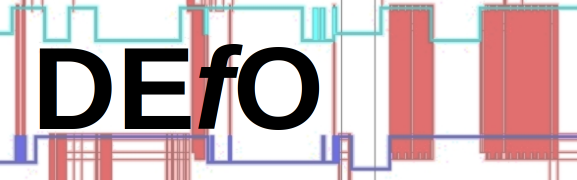
\includegraphics[width=4cm,keepaspectratio]{defologo.png}

\title{
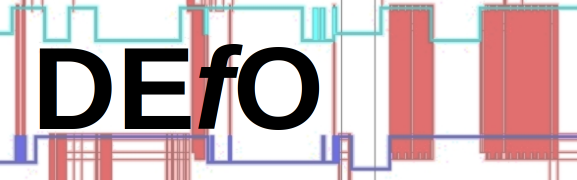
\includegraphics[width=\textwidth]{defologo.png}
ECH Interoperability Report}

\author{
\thanks{
Stephen Farrell is with Trinity College, Dublin 2, Ireland (email: stephen.farrell@cs.tcd.ie, https://www.cs.tcd.ie/Stephen.Farrell/)
}

\IEEEauthorblockN{Stephen Farrell}
\IEEEauthorblockA{
\\
	Trinity College Dublin/Tolerant Networks Ltd.\\
	stephen.farrell@cs.tcd.ie\\
	work-in-progress
}
}

%%\numberofauthors{1}

%%\author{\\
%%\alignauthor Stephen Farrell\\
%%    \affaddr{Trinity College Dublin}\\
%%	\email{Stephen.Farrell@cs.tcd.ie}}
%%}
%%}


%\date{}

%%\IEEEpubid{0000--0000/00\$00.00~\copyright~2016 IEEE}
\maketitle


\input abstract
\begin{IEEEkeywords}
Encrypted Client Hello (ECH), Interoperability
\end{IEEEkeywords}
\input introduction

% regular IEEE uses singular form of ACK (and no section #)
\input acks

\bibliographystyle{IEEEtran}
\bibliography{IEEEabrv,bib,ietf}

\end{document}
